\appendix

\sect{Tree Structure}

\subsect{Flattening}

A tree can be flattened for root-first traversal based on either breadth-first search (BFS) or depth first search (DFS).

\begin{itemize}
	\item $i$ is the zero-indexed traversal order, corresponding to an array
	index of the flattened tree.
	\item $m$ is the branching factor of the tree.
	\item $h$ is the height of the tree.
	\item $r$ is the ``row'' where a given node resides in the tree;
	the number of tree levels removed from the root.
	\item $c$ is the ``column'' where a given node resides  in the tree;
	the number of nodes away from the left edge.
\end{itemize}


\subsubsect{BFS}

$$
	i = \left\lfloor\sum_{k=1}^r m^k \right\rfloor + c
	= \left\lfloor\frac{1 - m^r}{1 - m}\right\rfloor + c
$$

\begin{figure}[H]
	\centering
	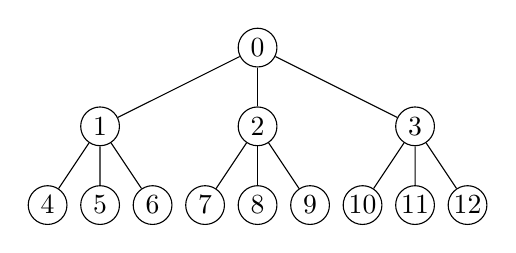
\begin{tikzpicture}[
			xscale=1.2,
			tree/.style={draw,circle,inner sep=0.25mm, minimum size=14pt}
		]
		\node[tree] at (0, 0) (00) {0};
		\foreach \r [
			evaluate = \r as \w using int(3^\r),
			evaluate = \r as \wl using int(3^\r-1)
		] in {1,...,2} {
			% Columns
			\foreach \c [
				evaluate = \c as \i using int((\w-1)/2 + \c),
				evaluate = \c as \pr using int(\r-1),
				evaluate = \c as \pc using int(\c/3),
			] in {0,...,\wl} {
				\node[tree] (\r\c)
					at ({(\c-int(\w/2)) / (\w/5)}, -\r) {\i};
				\draw[-] (\pr\pc) -- (\r\c);
			}
		}
	\end{tikzpicture}
\end{figure}


\subsubsect{DFS}

\begin{figure}[H]
	\centering
	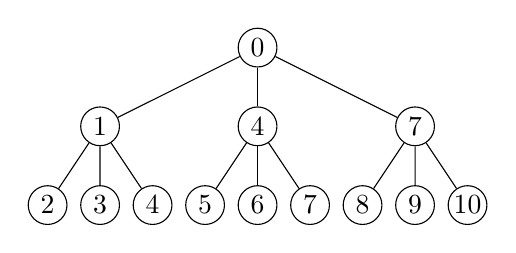
\begin{tikzpicture}[
			xscale=1.2,
			tree/.style={draw,circle,inner sep=0.25mm, minimum size=14pt}
		]
		\node[tree] at (0, 0) (00) {0};
		\foreach \r [
			evaluate = \r as \w using int(3^\r),
			evaluate = \r as \wl using int(3^\r-1)
		] in {1,...,2} {
			% Columns
			\foreach \c [
				evaluate = \c as \i using int(\r + \c*(3^(2-\r))),
				evaluate = \c as \pr using int(\r-1),
				evaluate = \c as \pc using int(\c/3),
			] in {0,...,\wl} {
				\node[tree] (\r\c)
					at ({(\c-int(\w/2)) / (\w/5)}, -\r) {\i};
				\draw[-] (\pr\pc) -- (\r\c);
			}
		}
	\end{tikzpicture}
\end{figure}
